\documentclass[10pt,twocolumn,letterpaper]{article}

\usepackage{cvpr}
\usepackage{times}
\usepackage{epsfig}
\usepackage{graphicx}
\usepackage{amsmath}
\usepackage{amssymb}
\usepackage{algorithm}
\usepackage{algorithmic}

% Include other packages here, before hyperref.

% If you comment hyperref and then uncomment it, you should delete
% egpaper.aux before re-running latex.  (Or just hit 'q' on the first latex
% run, let it finish, and you should be clear).
\usepackage[breaklinks=true,bookmarks=false]{hyperref}

\cvprfinalcopy % *** Uncomment this line for the final submission

\def\cvprPaperID{****} % *** Enter the CVPR Paper ID here
\def\httilde{\mbox{\tt\raisebox{-.5ex}{\symbol{126}}}}

% Pages are numbered in submission mode, and unnumbered in camera-ready
%\ifcvprfinal\pagestyle{empty}\fi
\setcounter{page}{1}
\newcounter{boldifyCounter}
\newcounter{fixmeSectionCounter}
\newcounter{fixmeTotalCounter}

%%%%%%%%%%%%% Drafting commands %%%%%%%%%%%%%%%%%%%%%%

\newcommand{\boldify}[1]{%
\stepcounter{boldifyCounter}%
\textbf{{\color{green}**}%
~\arabic{section}.\arabic{subsection}.\arabic{boldifyCounter}%
: #1}}

\newcommand{\FIXME}[1]{%
\stepcounter{fixmeSectionCounter}\stepcounter{fixmeTotalCounter}%
{\color{red}
\fbox{\color{black}%
\parbox{\linewidth}{%
\textbf{FIXME \arabic{section}.\arabic{subsection}.\arabic{fixmeSectionCounter} (\color{red}\#\arabic{fixmeTotalCounter}):} #1}}
}
}

\newcommand{\FIXED}[2]{%
{\color{blue}
\fbox{%
\parbox{\linewidth}{%
\textbf{FIXED \##1:} \color{black}#2}}
}
}


\addtocounter{fixmeSectionCounter}{-2}
\addtocounter{fixmeTotalCounter}{-2}
\makeatletter
\@addtoreset{fixmeSectionCounter}{section}
\@addtoreset{fixmeSectionCounter}{subsection}
\@addtoreset{boldifyCounter}{section}
\@addtoreset{boldifyCounter}{subsection}
\makeatother

\begin{document}

%%%%%%%%% TITLE
\title{Big Boards Mean Big Problems:\\ Solving M-N-K Games with Deep Reinforcement Learning}

\author{Jonathan Dodge,  Amrita Sadarangani,  Andrew Anderson\\
Oregon State University\\
Corvallis, OR\\
{\tt\small \{ dodgej, sadarana, anderan2 \} @oregonstate.edu }
% For a paper whose authors are all at the same institution,
% omit the following lines up until the closing ``}''.
% Additional authors and addresses can be added with ``\and'',
% just like the second author.
% To save space, use either the email address or home page, not both
}

\maketitle
%\thispagestyle{empty}

%%%%%%%%% ABSTRACT
\begin{abstract}
$M$-$N$-$K$ games are those that are played on a board of size $M$ by $N$ and won by forming a sequence of length $K$.
Such games include the likes of connect-4 or tic-tac-toe, and for smaller boards, winning tactics are well established.
However, as the board and sequence for winning grows larger, it becomes more complicated to determine a strategy that will lead to victory.
This paper looks at how deep reinforcement learning can be applied to effectively select moves in the large action space of $M$-$N$-$K$ games.
\end{abstract}

\section{Introduction}

\begin{figure}[b]
	\centering
	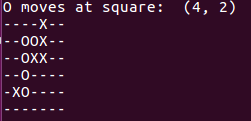
\includegraphics[ width = \columnwidth ]{Assets/argmax_9}
	\caption{ The board representations that the user sees on output }
	\label{fig:argmax_10}
\end{figure}

$M$-$N$-$K$ games are a popular method of entertainment, played by people of all ages.
They derive their name from being played on boards of size $M \times N$, and they are won by forming a sequence of length $K$.
Popular forms of these games are Tic-Tac-Toe and Connect 4, which would be a (3, 3, 3) and (6, 7, 4) $M$-$N$-$K$ game respectively.
Wei ji Ma~\cite{weiJiMa} discusses $M$-$N$-$K$ games and lists out the problems that have been ``solved\footnote{By ``solved'' we mean that it is known whether the first player to act will win or draw given optimal play from both sides.}'' in this domain.
He provides a table describing the regimes of $M$, $N$, and $K$ which are known to be solved, shown in Table~\ref{weiJiMa}.
This is where deep learning can really assist humanity in trying to show what conditions are viable for victory as the board size grows.

\begin{table}
\begin{tabular}{@{}l|l}
\emph{\textbf{$K$ values}} & Win on \emph{\textbf{$ M \times N$ board}} \\
\hline
1 & Always\\
\hline
2 &  iff $n > 2$\\
\hline
3 &  iff $m \geq 3$ and $n \geq 4$\\
\hline
4 & iff ($m \geq 5$ and $n \geq 6$) or ($m = 4$ and $n \geq 9$)\\
\hline
5 & if $m = n \geq 15$; not if $n \leq 6$ \\
\hline
6 & not if $m = n = 6$ (conjecture: never)\\
\hline
7 & (conjecture: never)\\
\hline
$\geq$ 8 & never \\
\end{tabular}
\caption{Wei Ji Ma's table describing solved states of MNK games.
Some results have been proven, and others are labelled conjectures}
\label{tab:weiJiMa}
\end{table}

From work such as AlphaGo Zero~\cite{alphaGoZero}, DeepMind has found a set of new opening moves that grandmasters in the domain of Go had not even considered viable opening moves.
However, the successes in this domain have shown that networks can see patterns and potential moves that even the strongest human players may not consider.
The problem with neural networks is that the solutions that they arrive at might not be understandable to humans, and this causes a problem when a human is asked to evaluate whether or not the network is making decisions \emph{for the right reasons}.

Approaching the $M$-$N$-$K$ games domain, we hope to work towards answering a few things that will help understanding the $M$-$N$-$K$ domain as well as help improve human-understanding of neural networks.
We wanted to:
\begin{enumerate}\itemsep0em
\item Investigate if a neural network can form winning strategies (particularly for larger boards which are not known to be solved).
\item Look at how different agents performed in this domain.
Our project created both search-based and CNN-based agents.
\item Use these agents to test human-understandability of explanations and network architectures.
\end{enumerate}

\section{Background}

Work in the $M$-$N$-$K$ domain for neural networks seems to be limited to the applications of tic-tac-toe, which is an example of a 3,3,3 game in $M$-$N$-$K$.
As early as 1993, evolutionary programming was utilized to create neural networks capable of playing tic-tac-toe~\cite{fogel1993using}.
Their work formed showed that when the domain was small, evolutionary programming was able to adjust architecture and connections of the single hidden layer perceptrons to adapt behavior when provided a given goal.

Grim et al.~\cite{grim2005probabilistic} performed their work also in a variant of tic-tac-toe, and they used probabilistic neural networks (PNN) to estimate distribution mixtures from training data through the Expectation-Maximization (EM) algorithm.
They varied the tic-tac-toe game by allowing the network to play on a $7 \times 7$ board, which means that the penalty of a wrong move is not so harsh as it is on a $3 \times 3$ board.
Their PNN approximates the class-conditional probability distributions by finite mixtures to use Bayesian decision-making.
Their training data was the use of a simple heuristic player as a teacher, generating the training data by ``observing'' the self-play of the heuristic player repeatedly.
Our work diverges from this by allowing the agents to learn by playing each other repeatedly, rather than having imitation learning.
Ultimately, Grim et al.~\cite{grim2005probabilistic} showed that a sequentially trained PNN was capable of learning complex decision-making in a 7,7,3 game.
Their work forms a good basis to model our human interpretable issue with, since they visualized the probabilities that the model was computing in grayscale, where the lighter the color indicated the less likely a move was to create a victory.

Probably the most similar work to our own is Greydanus et al.~\cite{greydanus}, where RL is applied to the Atari domain.
The major difference from our work is that the domains are different, with a much larger action space in our domain, since Atari only has 8 directions + button pressed (or not) amounting to 16 actions for all states in all games.
The $M$-$N$-$K$ game domain has a much larger action space, and we are not working from pixels on the game screen.
Nonetheless, the code hosted on Greydanus et al.'s github repo was helpful in producing our results

Our approach differs from the existing methods because we apply the CNN architecture.
Additionally, we are applying reinforcement learning techniques in order to allow for the agent to have the potential to succeed with boards beyond $3 \times 3$ where the state space can be enumerated and correct actions specified for each state.
Thus, the tic-tac-toe case corresponds to a case of \emph{imitation learning}, which we want to expand beyond.
\section{Technical Approach}

We began by building a simulator for general $M$-$N$-$K$ games.
We started with a very simple agent \texttt{RandomAgent} -- which simply gathered the set of legal moves and chose randomly between them.
This agent allowed us to test the simulator and would become the backbone of our next agent -- \texttt{SearchAgent}.

\subsection{Search-based Agents}

\textbf{The \texttt{SearchAgent}} uses a search algorithm that resembles Monte Carlo Tree Search (MCTS), which we call Nearly MCTS (NMCTS).
Chaslot et al. wrote a paper about MCTS and its usefulness for solving board games of the modern and classic variety, as well as even video games~\cite{chaslot2008monte}.
Given a board at timestep $t$, the agent again collects the set of legal moves and then performs 1 step of search by copying the board and ``imagining'' making each legal move -- generating a board at timestep $t+1$.
This board is then used by 2 \texttt{RandomAgent}s to compute a set number of random rollouts to a terminal state.
Using the set of wins/losses/draws from the random rollouts, the \texttt{SearchAgent} now has an estimate of the quality of the state that results from selecting each action.

\begin{algorithm}
\caption{SearchAgents::move(board)}
\begin{algorithmic}[1]
\STATE{estWins = []}
\STATE{estLosses = []}
\STATE{estDraws = []}
\FOR{($i$,$j$) in availSquares}
\STATE{wins = losses = draws = $0.0$}
\FOR{games in numGamestoEstimate}
\STATE{Create deep copy of board}
\STATE{Add piece to ($i$,$j$) in copy}
\STATE{Play random game from here}
\IF{Win game}
\STATE{wins $\leftarrow$ wins + 1}
\ELSIF{Lose game}
\STATE{losses $\leftarrow$ losses + 1}
\ELSE{}
\STATE{draws $\leftarrow$ draws + 1}
\ENDIF{}
\ENDFOR{}
\STATE{Append wins to estWins}
\STATE{Append losses to estLosses}
\STATE{Append draws to estDraws}
\ENDFOR{}
\STATE{MoveScores = $2 \times wins - losses + draws$ }
\RETURN{availSquares( argmax( moveScores ) )}
\end{algorithmic}

\end{algorithm}

\subsubsection{Search-based Action Selection}

However, given a 3-element tuple of wins/losses/draws, selecting an action is not so easy!
For example, we specified that the agent should select the \texttt{argmax\{ estimatedWin \}}, which resulted in a very aggressive agent that was singularly focused on forming its sequence and disregarded the other agent's actions.
This resulted in games where the agent would be second to act, but still choose to race its opponent rather than defend.

\begin{figure}
	\centering
	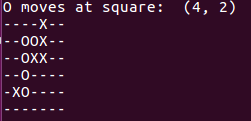
\includegraphics[ width = \columnwidth ]{Assets/argmax_9}
	\caption{A Sample of a Search-Based Agent's roll-outs as probabilities }
	\label{fig:argmax_1}
\end{figure}

So, we also varied our agent's approach to select the \texttt{argmin\{ estimatedLosses \}}, which led to a very defensive agent that usually played to a draw.
These agents were so focused on blocking any sequence of their enemy that they did not seem to want to form a sequence of their own.
To illustrate, we observed that when the agent was first to act, it would choose to defend its opponent rather than race to complete a sequence.
We hypothesized that some linear combinations of win, loss, and draw probabilities might make for a more effective agent, so we developed the equation:
\emph{Score = 2 * Win - Loss + Draw}
When we tested \texttt{argmax\{ Score \}}, we noticed that the behavior was almost identical to the \texttt{argmin\{ estimatedLosses \}}.

\subsection{The Neural Network Agent}

We wanted to compare the \texttt{SearchAgent} to one that uses a neural network to compete.
We call this agent the \texttt{nnAgent}, and its architecture follows that the input, the board, is passed through 
some convolutional layers, each with a 3x3 filter with padding.
Once the board has passed through these convolution layers, it is then passed through a fully connected layer with M * N outputs.
These output are then passed through two linear layers, the \emph{critic} and the \emph{actor}.
The critic takes the board size units and outputs one unit.
This estimates the value of the current state, under the assumption that the agent will behave according to the same policy in the future.
The actor, however, takes the board size (M * N) as input and has M * N outputs.
The actor selects the output unit that is most activated (via softmax), and that becomes the \texttt{nnAgent}'s move.

\begin{figure}
	\centering
	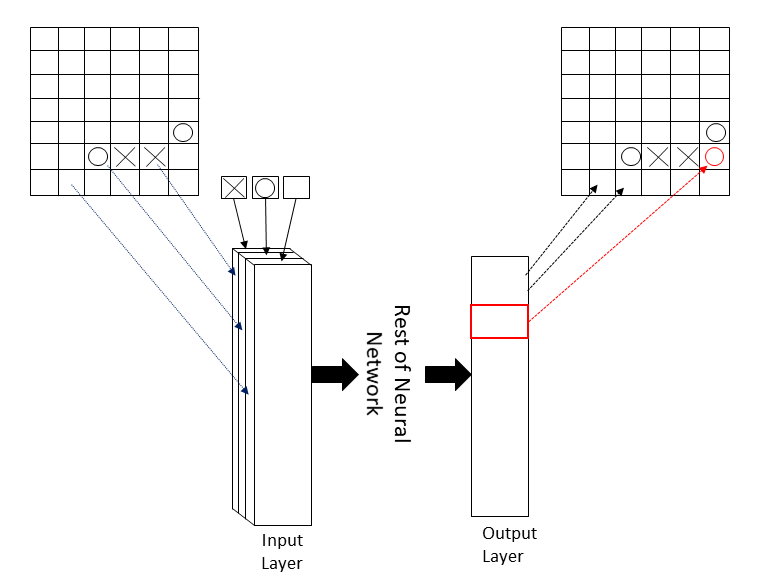
\includegraphics[width = \columnwidth, height = 70mm]{Assets/NetworkArchitecture3}
	\caption{The architecture of the CNN agent that plays, up until the actor/critic stage
    }
    \vspace{-4mm}
\label{fig:networkArchitecture}
\end{figure}

\begin{algorithm}
\caption{nnAgent(squareType, m, n, k)}
\begin{algorithmic}[1]
\STATE{nn.Conv2d(chans, c1Outs, kern, pad=int(kern/2))}
\STATE{nn.Conv2d(c1Outs, c2Outs, kern, pad=int(kern/2))}
\STATE{nn.Linear(c2Outs * m * n, m * n)}

\STATE{actor = nn.Linear(m * n, m * n)}
\STATE{critic = nn.Linear(m * n, 1)}
\end{algorithmic}

\end{algorithm}

\subsubsection{Training, Rewards, and Targets}

We used reinforcement learning to train the network.
If an agent tries to make an invalid move, such as trying to lay their glyph over an occupied spot, then a strong negative reward is given immediately.
In addition, the agent performs a weight update and is given another chance to make a legal move (up to a fixed number of tries, currently set at 300).
If the number of tries is exceeded, the agent reports the illegal move provided by the network, and the simulator will ignore it.
In essence, if the network fails to provide a legal move in a good number of tries, it loses its turn.

Once a game is complete, a reward is obtained.
A positive reward is obtained for the agent that wins, and a negative reward is obtained for the agent that loses.
If there is a draw, there is a smaller positive reward given to both agents.
Using this reward, we generate a target by taking a forward step, capturing the NN outputs, using them to determine the selected action, then modifying the target activation level \emph{for ONLY that action} by adding the reward to it.
The target values for the non-selected actions remains the same as the NN's output.
Thus, there is always loss in the network, because when the agent observes positive, pulling the target activation down will serve to reduce the probability that action is selected (and vice versa for negative reward).
The loss function we used was the Smooth-L1 loss, which is also known as least absolute errors.
It takes an output and target which are the same shape, which is ideal for our circumstances, where the lack of a ``true label'' rules out using something like cross entropy.

\begin{algorithm}
\caption{nnAgent::observeReward(history, reward)}
\begin{algorithmic}[1]
\STATE{Create Optimizer}
\STATE{Split history into just boards}
\FOR{board in history}
\STATE{nnOutput = forwardPass(board)}
\STATE{actionIdx = argmax(softmax(nnOutput))}
\STATE{target = nnOutput}
\STATE{target[actionIdx] += reward}
\STATE{loss = SmothL1Loss()(nnOutput, target)}
\STATE{backwardPass and update weights}
\ENDFOR{}
\end{algorithmic}

\end{algorithm}

\subsubsection{Stabilizing the Gradient}

Since our approach does not use any kind of memory replay (as done in~\cite{pytorchTut}), our gradient estimations can be very noisy.
One of the main extensions that would benefit our project is implementing a batch-mode gradient update using uncorrelated samples.
Currently, we are updating using the gradient from 1 complete action history, which is correlated.
We would like to store a database of the agent's experiences anyway, since querying it could be useful for explanation, in addition to improving gradient estimation. 
Our network uses the Adam optimizer with a learning rate of 1e-3 and a weight decay of 1e-4.
\section{Experiment Design and Results}

\subsection{Experiment Design}

Since our project was focused on the NN-based agents, we set up our experiments to test its performance as we trained it in the following way.
The \texttt{nnAgent} being tested, call it \texttt{ourHero}, will train against a \texttt{SearchAgent} as a sparring partner for a specified number of games.
Then, we perform a test, which corresponds to \texttt{ourHero} facing each opponent in a gauntlet in a specified number of games, with output reported.
(Note that we do not halt weight updates during testing, so we have a slight distinction from the traditional train/test separation).
As this process is repeated for a large number of testing sessions, we report win/loss/draw count, \# of illegal moves, maximum game length (in moves) and average game length (also in moves).
Note that since we executed all this code on CPUs, not GPUs, our network is not very deep since we could not devote a great deal of compute to training.
Similarly, the \texttt{SearchAgent} does very few rollouts -- merely 5 (as we achieve better performance we can add agents which perform more accurate value estimation to the gauntlet).


\subsection{Results}
We wanted to sample from the amount of time that the agent had had to train before going into the gauntlet.
We hypothesized that the more time that the agent had had to train before entering, the better that it would perform against the opposing agents.
However, we were surprised to learn that the agent performed \emph{decreasingly} better as the amount of training games increased.
\begin{table}
\begin{tabular}{@{}p{.18\columnwidth}|p{.4\columnwidth}|p{.33\columnwidth}}
\hline
Training Games & Random Agent (Win\%) & Bad Search(Win\%)\\
\hline
50 & 83 & 13 \\
\hline
100 & 74 & 15\\
\hline
150 & 75 & 13\\
\hline
200 & 69 & 16\\
\end{tabular}
\vspace{2pt}
\caption{ Using the Adam optimizer, we used a learning rate of 1e-3 and a weight decay of 1e-4 to obtain these results. The total number of games tested was 100, so the percentages (the right two columns) were computed by $(numWins/numGames)\times 100$ }
\label{tab:results}
\end{table}

%\begin{figure}[b]
	\centering
	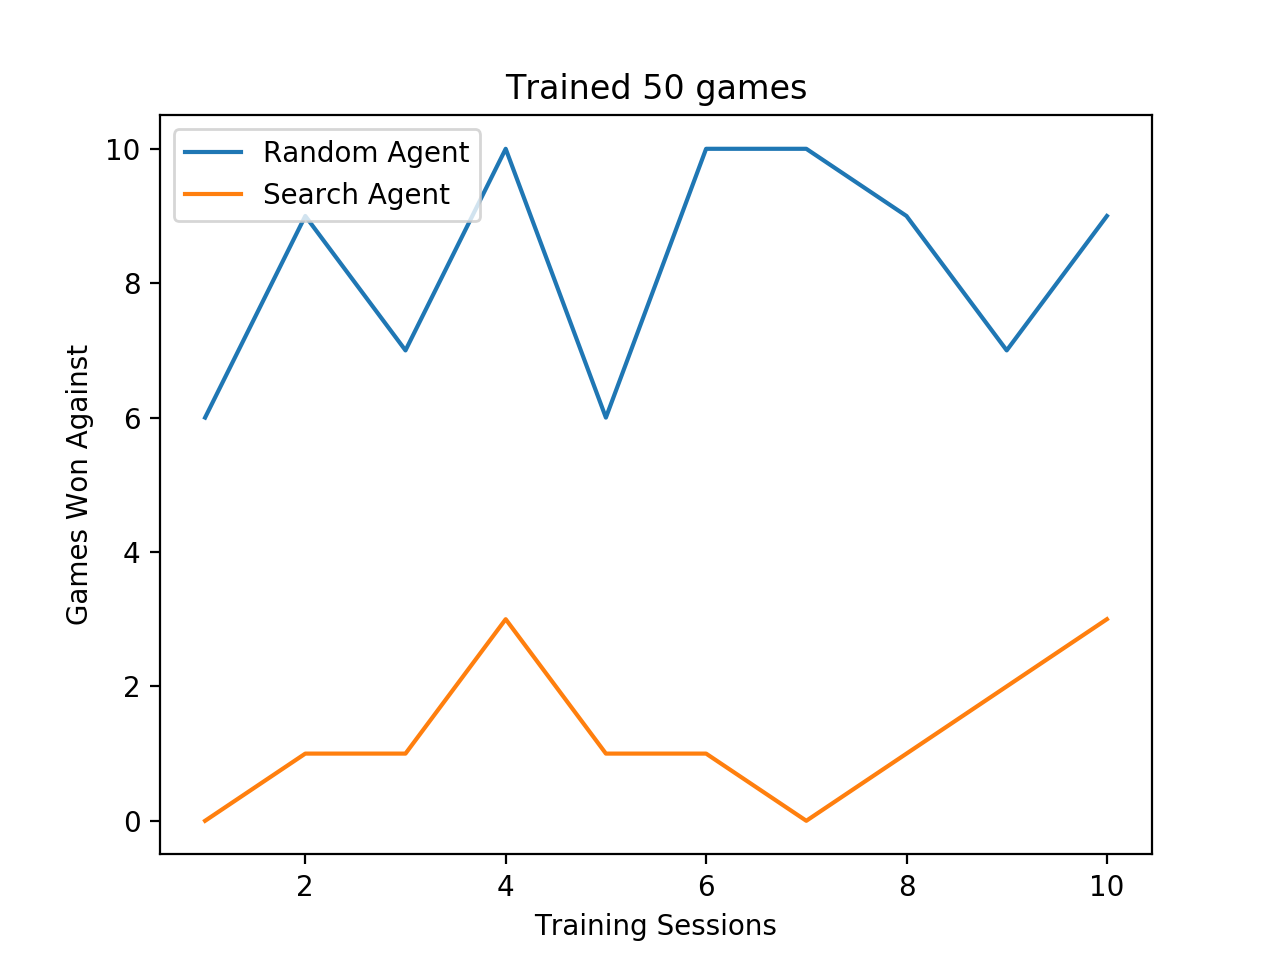
\includegraphics[ width = \columnwidth ]{Assets/50TrainedGames}
	\caption{Our results from when the sampling occurs after 50 training sessions}
	\label{fig:50TrainResults}
\end{figure}
\begin{figure}[b]
	\centering
	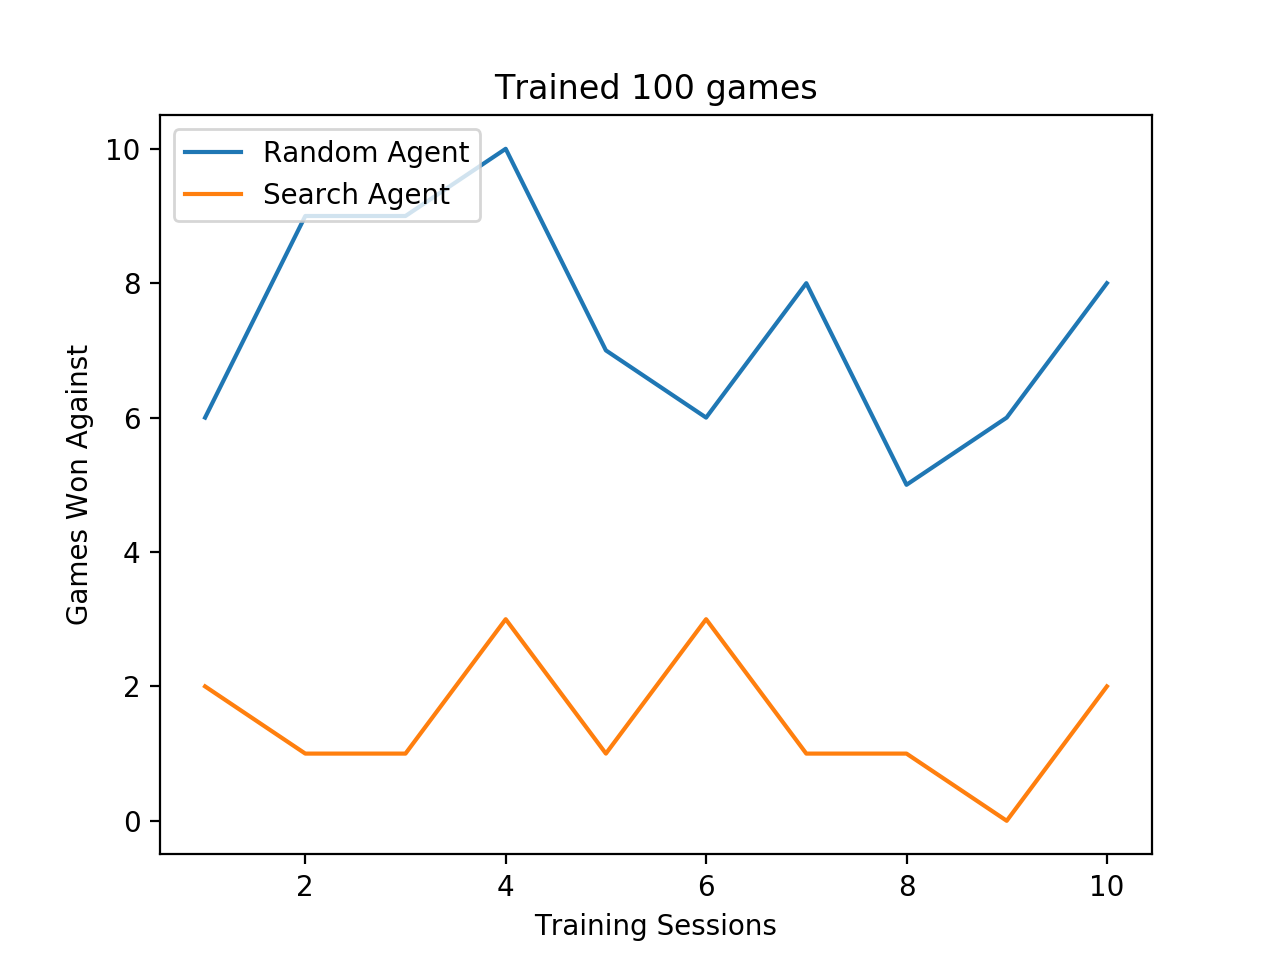
\includegraphics[ width = \columnwidth ]{Assets/100TrainedGames}
	\caption{Our results when sampling over each 100 sessions. What we noted during this was initially increasing behavior against the random agent, which turned into worse behavior as time went on.}
	\label{fig:100TrainedResults}
\end{figure}
\begin{figure}[b]
	\centering
	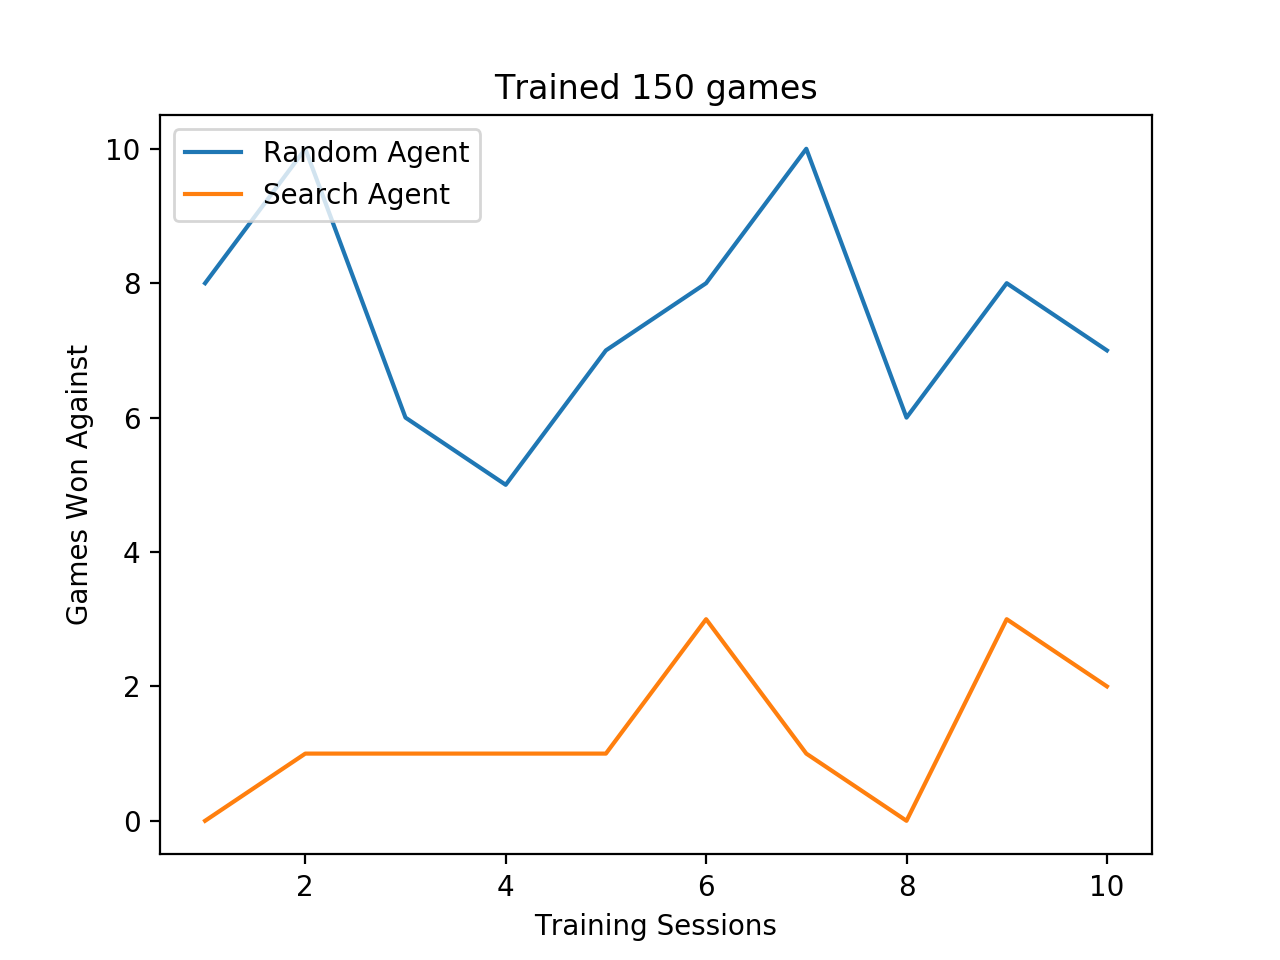
\includegraphics[ width = \columnwidth ]{Assets/150TrainedGames}
	\caption{We noticed a far more erratic behavior for the agent when it was tested after every 150 games. Initially, it performed well, but the sharp decrease came much quicker than in previous cases. When it came to the Search-Based agent, there was far more stable data coming in.}
	\label{fig:150TrainedResults}
\end{figure}
\begin{figure}[b]
	\centering
	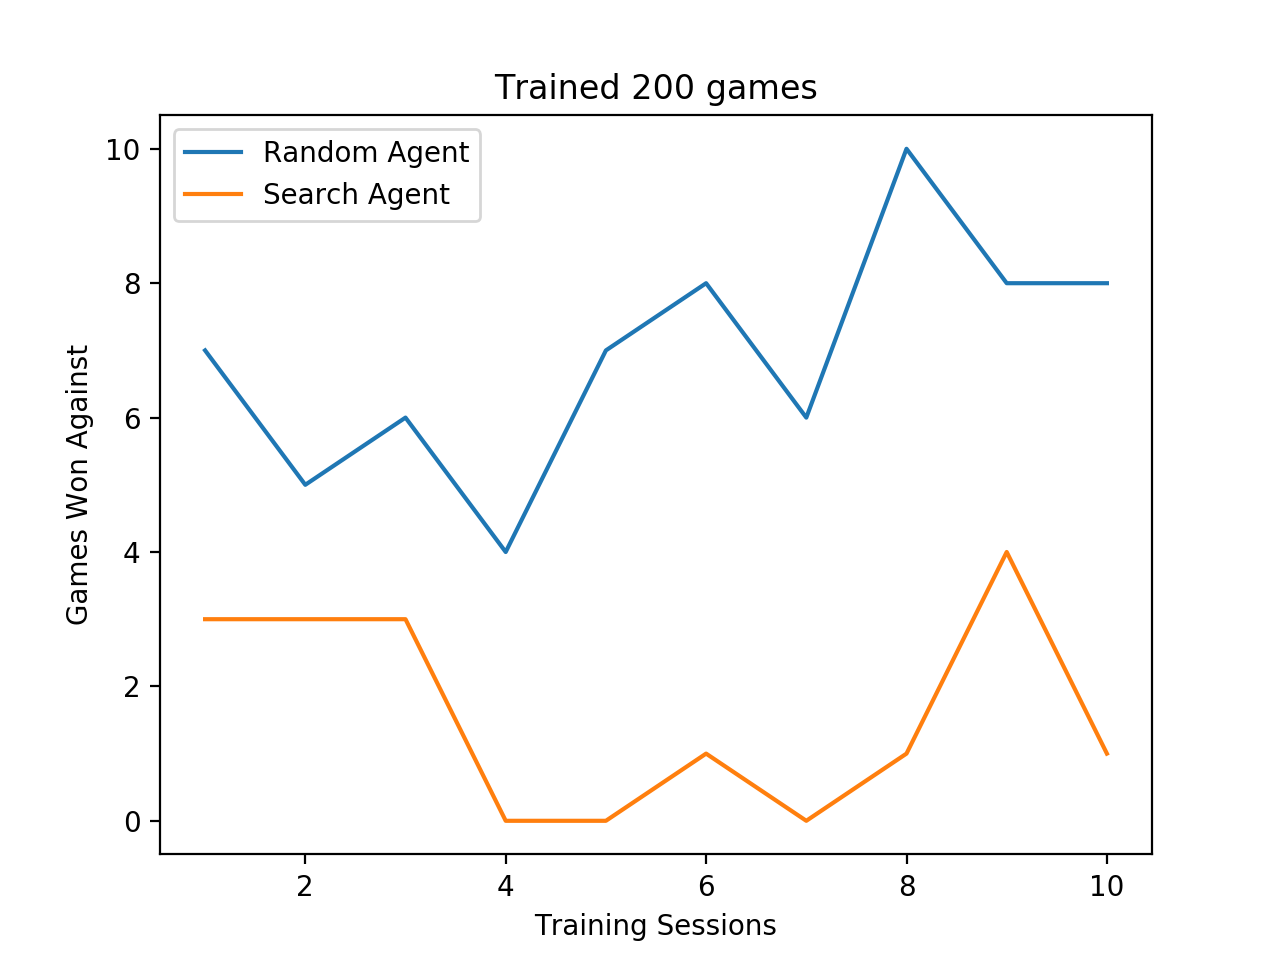
\includegraphics[ width = \columnwidth ]{Assets/200TrainedGames}
	\caption{When it came to 200 training samples before testing, our agent showed an increasing performance against opposing agents. With more computing resources, like the ability to run the code on GPUs, we hope to see that this trend increases as the number of training samples before testing increases.}
	\label{fig:200TrainedResults}
\end{figure}
\begin{figure}[b]
	\centering
	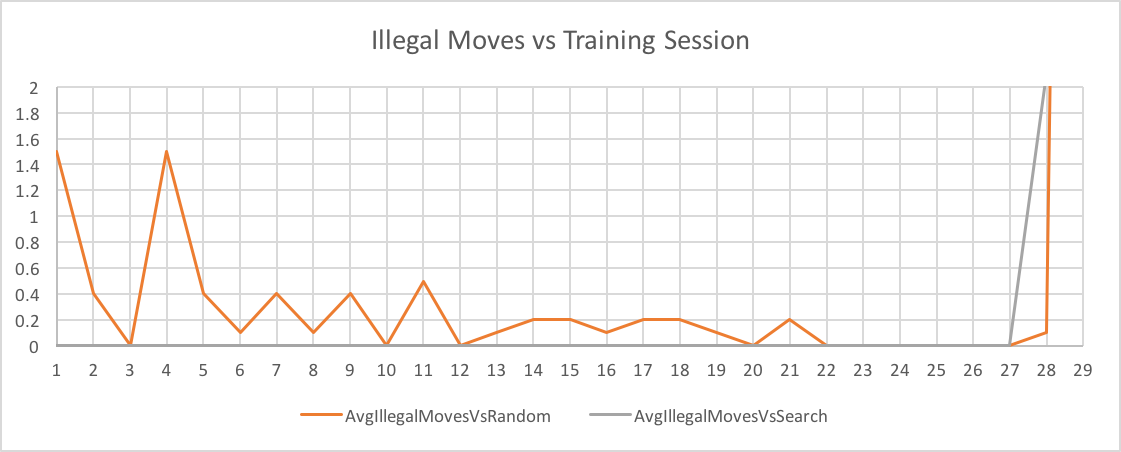
\includegraphics[ width = \columnwidth ]{Assets/pic_png-3}
	\caption{Illegal moves vs training session.  Note how initially the \# of illegal moves is fairly high, then quickly drops to zero.
    Notably, after many training sessions of 0 illegal moves, we observe a spike in the number of illegal moves around training session 28.}
	\label{fig:IllegalMovesTraining}
\end{figure}
\begin{figure}[b]
	\centering
	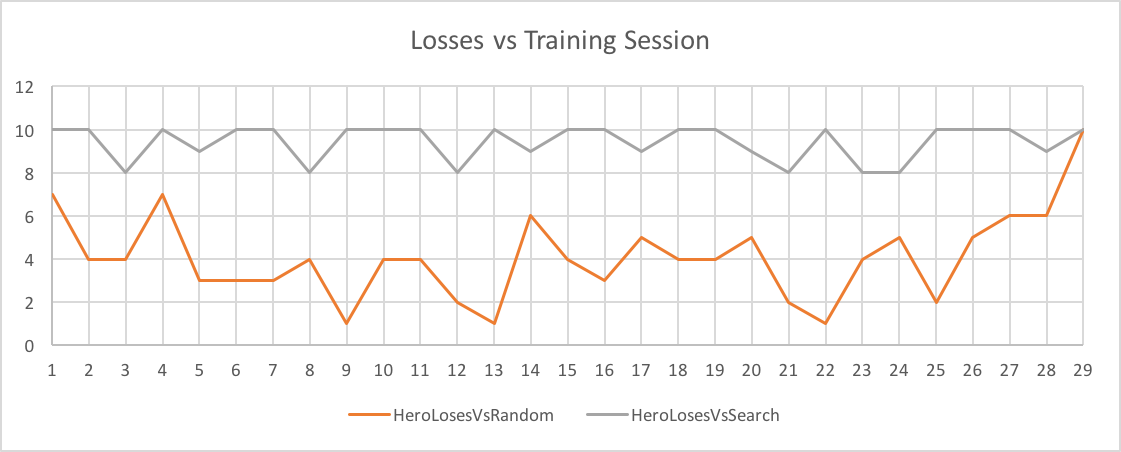
\includegraphics[ width = \columnwidth ]{Assets/pic_png-2}
	\caption{Loss count vs training sessions.
    Note that loss count drops initially, then rises again.
    Particularly, note how sharply the loss count rises as the training session approaches 28.
    We found that with these training sessions, win rate (and illegal moves) really went haywire around training session 28, which indicates noise in the gradient.
   	As described earlier, minibatch-based training is likely the best remedy for this behavior.}
	\label{fig:LossesvTraining}
\end{figure}
\begin{figure}[b]
	\centering
	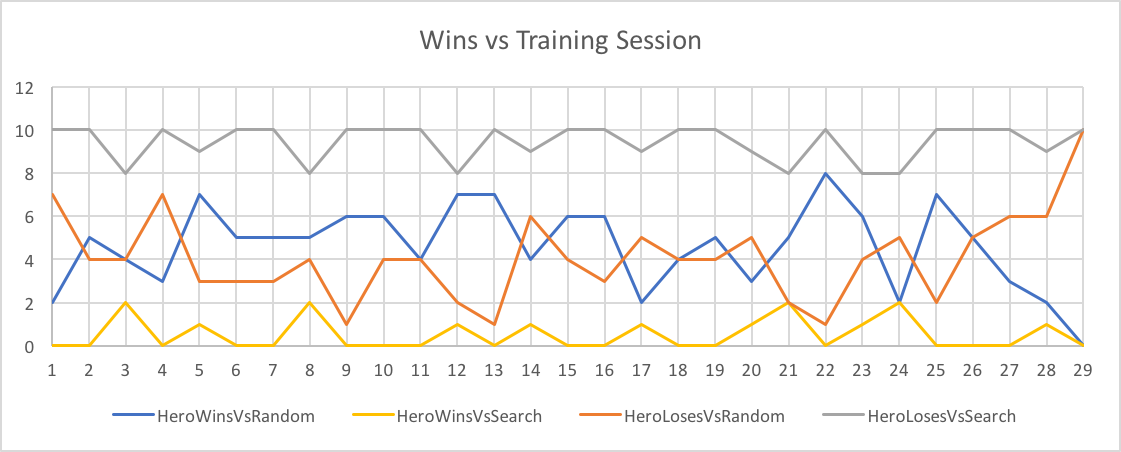
\includegraphics[ width = \columnwidth ]{Assets/pic_png-1}
	\caption{Win (and draw) count vs Training sessions.  Note that wins/losses do not change all that much over the course of training.
    Notably, after the first few training sessions, the maximal (or near it) values for win/draw counts have ben observed}
	\label{fig:WinsvTraining}
\end{figure}





\section{Conclusion and Future Work}

In this paper, we have presented our approach to building convolutional neural network-based agents to play $M$-$N$-$K$ games.
We used reinforcement learning to train our agents, and reported some preliminary results on their performance vs some baseline agents.

For future work, we would like to implement an LSTM architecture for an agent.
This would give us a look at the impact of memory on the performance of the agent.
We would also like to optimize the architecture of the CNN-Agent -- in particular, we are curious to know if matching the kernel sizes to $K$ has benefits in performance, network size, training time, and human understandability.

We also want to learn what it means for a network to be understandable to humans.
This platform can be used to compute and present saliency maps for selected moves.
Testing these types of visualizations with human participants to see if they can pick the strongest agent would be very interesting.
Another type of explanation we would like to work towards is one relative to training data. 
Namely, when a CNN generates an output, it does so in the context of all the other inputs it has ever seen.
Thus, when a behavior is avoided by the network, it has encoded a great deal of painful experience into the configuration of the network.
Revealing the reason for this configuration to the human will likely require references relative to previously observed states.


\clearpage
\bibliographystyle{ieee}
\pagestyle{plain}
\bibliography{egbib}

\end{document}
